\section{Anexos}

\subsection{Fragmentos de codigo}

\subsubsection{Plotter}---

\subsubsection{Colores}---

\begin{lstlisting}[language=C, caption={Librerias utilizadas}]
#define F_CPU 16000000UL

#include <avr/io.h>
#include <util/delay.h>
#include <avr/interrupt.h>
#include <string.h>
\end{lstlisting}

\begin{lstlisting}[language=C, caption={Mapeado de colores}]
typedef struct {
	const char *name;
	uint16_t r, g, b;
} ColorRef;

const ColorRef color_refs[] = {
	{"MORADO",    216, 157, 274},
	{"ROJO",       206, 149, 262},
	{"AMARILLO",    196, 99, 105},
	{"VERDE",     272, 192, 152},
	{"AZUL CLARO", 151, 153, 122},
	{"VIOLETA",    253, 275, 338},
	{"BLANCO",    110, 93, 91},
};
\end{lstlisting}

\begin{lstlisting}[language=C, caption={Convertidor de unsigned integer a string}]
// Convierte un valor entero sin signo en un string
void UTOA(uint16_t value, char *buffer) { 
	char temp[6];
	int i = 0, j = 0;

	if (value == 0) {
		buffer[0] = '0';
		buffer[1] = '\0';
		return;
	}

	// Convert digits to temp buffer (reversed)
	while (value > 0 && i < sizeof(temp) - 1) {
		temp[i++] = (value % 10) + '0';
		value /= 10;
	}

	// Reverse digits into final buffer
	while (i > 0) buffer[j++] = temp[--i];
	buffer[j] = '\0';
}
\end{lstlisting}

\begin{lstlisting}[language=C, caption={Enviado de datos a tira LED}]
void send_bit(uint8_t bitVal){
	if(bitVal){
		PORTD |=  (1<<LED_PIN);
		asm volatile (
		"nop\n\t""nop\n\t""nop\n\t""nop\n\t""nop\n\t"
		"nop\n\t""nop\n\t""nop\n\t""nop\n\t");
		
		PORTD &= ~(1<<LED_PIN);
		
		asm volatile (
		"nop\n\t""nop\n\t""nop\n\t""nop\n\t");
		
		} else {
		PORTD |=  (1<<LED_PIN);
		asm volatile (
		"nop\n\t""nop\n\t""nop\n\t");
		
		PORTD &= ~(1<<LED_PIN);
		asm volatile (
		"nop\n\t""nop\n\t""nop\n\t""nop\n\t""nop\n\t"
		"nop\n\t""nop\n\t""nop\n\t""nop\n\t""nop\n\t");
	}
}

// Envia un Byte a la tira de leds
// Utiliza cli y sei para un timing preciso
void send_byte(uint8_t byte) {
	cli();  
	for (uint8_t i = 0; i < 8; i++) {
		send_bit(byte & 0x80);  // send most significant bit first
		byte <<= 1;             // shift next bit into MSB position
	}
	sei();  // re-enable interrupts
}
\end{lstlisting}

\begin{lstlisting}[language=C, caption={Inicializadores}]
void usart_init(void) {
	const uint16_t ubrr = (16000000UL / (16UL * BAUD_RATE)) - 1;
	UBRR0H = ubrr >> 8;
	UBRR0L = ubrr;
	UCSR0A = 0;
	UCSR0B = (1 << TXEN0) | (1 << RXEN0) | (1 << RXCIE0);   // RX interrupt
	UCSR0C = (1 << UCSZ01) | (1 << UCSZ00);               // 8N1
}

void adc_init(void) {
	ADMUX  = (1 << REFS0);                        
	ADCSRA = (1 << ADEN)                          
	| (1 << ADPS2) | (1 << ADPS1) | (1 << ADPS0); // Prescaler 128
}

void rgb_init(void){
	DDRB |= (1<<RED) | (1<<GREEN) | (1<<BLUE);
}


void servo_init(void) {
	SERVO_DDR |= (1 << SERVO_PORT); 

	TCCR1A = (1 << COM1A1) | (1 << WGM11);
	TCCR1B = (1 << WGM13) | (1 << WGM12) | (1 << CS11); // 8

	ICR1 = 39999;   
}
 
void ws2812_init(void) { // tira de leds
	LED_DDR |= (1 << LED_PIN);
}
\end{lstlisting}

\begin{lstlisting}[language=C, caption={Funciones de utilidad}]
void ws2812_send_pixel(uint8_t r, uint8_t g, uint8_t b) {
	// Cambiar orden dependiendo de formato de tira led o matriz
	send_byte(g);
	send_byte(b);
	send_byte(r);
}

// Encender n leds del mismo color
void ws2812_fill(uint8_t r, uint8_t g, uint8_t b, uint16_t n) {
	cli(); 
	for (uint16_t i = 0; i < n; i++) {
		ws2812_send_pixel(r, g, b);
	}
	sei();
	ws2812_show();
}

// Establecer colores predeterminados
void led_strip_set_color(uint8_t color_id) {
	uint8_t r = 0, g = 0, b = 0;

	switch (color_id) {
		case 1: // Rojo
		r = 255; g = 0; b = 0;
		break;

		case 2: // Amarillo
		r = 255; g = 100; b = 0;
		break;

		case 3: // Verde
		r = 0; g = 255; b = 0;
		break;

		case 4: // Azul claro
		r = 0; g = 255; b = 255;
		break;

		case 5: // Violeta
		r = 100; g = 0; b = 100;
		
		break;

		case 6: // Morado
		r = 200; g = 0; b = 75;
		
		break;

		case 7: // Blanco
		r = 255; g = 255; b = 255;
		break;

		default: // Apagar LED
		r = g = b = 0;
		break;
	}

	ws2812_fill(r, g, b, 50);
}

// Establecer angulo en el servomotor
void servo_set_angle(uint8_t angle) {
	uint16_t pulse = 1000 + ((uint32_t)angle * 4000) / 180;
	OCR1A = pulse;
}

// Leer adc
uint16_t adc_read(uint8_t channel) {
	ADMUX = (ADMUX & 0xF0) | (channel & 0x0F);  
	ADCSRA |= (1 << ADSC);                     
	while (ADCSRA & (1 << ADSC));               // Wait for conversion to finish
	return ADC;                                 
}

// Establecer color del led rgb (iluminador)
void rgb_set(uint8_t r, uint8_t g, uint8_t b) {
	PORTB = (PORTB & ~((1 << RED)|(1 << GREEN)|(1 << BLUE))) |
	((r<<RED) | (g<<GREEN) | (b<<BLUE));
}

// Identificar color a partir de valores rgb.
// Tomando cada valor calibrado como un vector, se determina la distancia
// cartesiana del vector leido por el sensor.
const char* identify_color(uint16_t r, uint16_t g, uint16_t b) {
	uint32_t best_dist = 0xFFFFFFFF;
	const char *best_name = "UNKNOWN";

	for (uint8_t i = 0; i < NUM_COLORS; i++) {
		int32_t dr = (int32_t)r - color_refs[i].r;
		int32_t dg = (int32_t)g - color_refs[i].g;
		int32_t db = (int32_t)b - color_refs[i].b;
		uint32_t dist = dr*dr + dg*dg + db*db;

		if (dist < best_dist) {
			best_dist = dist;
			best_name = color_refs[i].name;
		}
	}
	return best_name;
}
\end{lstlisting}


\begin{lstlisting}[language=C, caption={Bucle principal}]
// programa principal
int main(void) {
	ws2812_init();
	usart_init();
	adc_init();
	rgb_init();
	servo_init();
	sei();
	
	while (1) {
		rgb_read();
		_delay_ms(50);

	
	}
}
\end{lstlisting}

\subsubsection{Piano}---


USART con buffers
\begin{lstlisting}[language=C, caption={Funciones USART con buffering}]

#define TX_BUF_SZ 128
#define TX_MASK   (TX_BUF_SZ - 1)

#define RX_BUF_SZ 128
#define RX_MASK   (RX_BUF_SZ - 1)

uint8_t tx_buf[TX_BUF_SZ];
uint8_t tx_head = 0, tx_tail = 0;

uint8_t rx_buf[RX_BUF_SZ];
uint8_t rx_head = 0, rx_tail = 0;

uint8_t usart_rx_available(void) {
	return (uint8_t)((rx_head - rx_tail) & RX_MASK);
}

void usart_init_9600(void) {
	const uint16_t ubrr = (16000000UL / (16UL * 9600)) - 1;
	UBRR0H = ubrr >> 8;
	UBRR0L = ubrr;
	UCSR0A = 0;
	UCSR0B = _BV(TXEN0) | _BV(RXEN0) | _BV(RXCIE0);   // <- RX interrupt
	UCSR0C = _BV(UCSZ01) | _BV(UCSZ00);               // 8N1
}

// USART
void usart_init_9600(void) {
	const uint16_t ubrr = (16000000UL / (16UL * 9600)) - 1;
	UBRR0H = ubrr >> 8;
	UBRR0L = ubrr;
	UCSR0A = 0;
	UCSR0B = _BV(TXEN0) | _BV(RXEN0) | _BV(RXCIE0);   // <- RX interrupt
	UCSR0C = _BV(UCSZ01) | _BV(UCSZ00);               // 8N1
}

// Escribir byte al buffer
uint8_t usart_write_try(uint8_t b) {
	uint8_t next = (uint8_t)((tx_head + 1) & TX_MASK);
	if (next == tx_tail) return 0;               // buffer lleno
	tx_buf[tx_head] = b;
	tx_head = next;
	UCSR0B |= _BV(UDRIE0);                       // kick the ISR
	return 1;
}

// Escribir string al buffer
uint16_t usart_write_str(const char *s) {
	uint16_t n = 0;
	while (*s && usart_write_try((uint8_t)*s++)) n++;
	return n;
}

// Leer byte del buffer de recepcion
uint8_t usart_read_try(uint8_t *b) {
	if (rx_head == rx_tail) return 0;                
	*b = rx_buf[rx_tail];
	rx_tail = (uint8_t)((rx_tail + 1) & RX_MASK);
	return 1;
}

// Interrupcion de registro de TX libre
ISR(USART_UDRE_vect) {
	if (tx_head == tx_tail) {                    
		UCSR0B &= (uint8_t)~_BV(UDRIE0);         
		return;
	}
	UDR0 = tx_buf[tx_tail];
	tx_tail = (uint8_t)((tx_tail + 1) & TX_MASK);
}

// Interrupcion de dato recibido
ISR(USART_RX_vect) {
	uint8_t d = UDR0;
	uint8_t next = (uint8_t)((rx_head + 1) & RX_MASK);
	if (next != rx_tail) {                
		rx_buf[rx_head] = d;
		rx_head = next;
	}
}
\end{lstlisting}

Formato de guardado de canciones
\begin{lstlisting}[language=C, caption={Guardado de canciones}]
// Midi tracks
// Generated using https://github.com/ShivamJoker/MIDI-to-Arduino
const int midiC[827][3] PROGMEM = {
	{E5, 94, 0},
	{B4, 94, 0},
	{A4, 94, 0},
	{E4, 94, 0},
	{A4, 94, 0},
	{B4, 94, 0}
    // ... 
}
\end{lstlisting}

\begin{lstlisting}[language=C, caption={Manejo de eventos RX USART}]
void handleUSART(uint8_t character){
	if (character == '1'){
		mode = 1;
		eventAoff = 1;
		eventBoff = 0;
		
		song = 0;
		
		eventAon = 0; // Encender track A
		indexA = 0; // Posicion track A
		countA = 0; // Conteo de overflow de notas de track A
		maxCountAon = 0; // Maximo conteo de overflow encendido en A
		maxCountAoff = 0; // Maximo conteo de overflow apagado en A
		enableCountAon = 0; // Habilitar conteo de encendido en A
		enableCountAoff = 0; // Habilidad conteo de apagado en A
		
		eventBon = 0; // Encender track B
		indexB = 0; // Posicion track B
		countB = 0; // Conteo de overflow de notas de track B
		maxCountBon = 0; // Maximo conteo de overflow encendido en B
		maxCountBoff = 0; // Maximo conteo de overflow apagado en B
		enableCountBon = 0; // Habilitar conteo de encendido en B
		enableCountBoff = 0; // Habilidad conteo de apagado en B
		
		PCICR &= ~((1 << PCIE1) | (1 << PCIE2));
		stopFrequencyB();
		
	} else if (character == '2'){
		mode = 1;
		eventAoff = 1;
		eventBoff = 1;
		
		song = 1;
		
		eventAon = 0; // Encender track A
		indexA = 0; // Posicion track A
		countA = 0; // Conteo de overflow de notas de track A
		maxCountAon = 0; // Maximo conteo de overflow encendido en A
		maxCountAoff = 0; // Maximo conteo de overflow apagado en A
		enableCountAon = 0; // Habilitar conteo de encendido en A
		enableCountAoff = 0; // Habilidad conteo de apagado en A
		
		eventBon = 0; // Encender track B
		indexB = 0; // Posicion track B
		countB = 0; // Conteo de overflow de notas de track B
		maxCountBon = 0; // Maximo conteo de overflow encendido en B
		maxCountBoff = 0; // Maximo conteo de overflow apagado en B
		enableCountBon = 0; // Habilitar conteo de encendido en B
		enableCountBoff = 0; // Habilidad conteo de apagado en B
		
		PCICR &= ~((1 << PCIE1) | (1 << PCIE2));
		stopFrequencyA();

	} else if (character == 'P'){
		mode = 0;
		eventAoff = 0;
		eventBoff = 0;
				
		eventAon = 0; // Encender track A
		indexA = 0; // Posicion track A
		countA = 0; // Conteo de overflow de notas de track A
		maxCountAon = 0; // Maximo conteo de overflow encendido en A
		maxCountAoff = 0; // Maximo conteo de overflow apagado en A
		enableCountAon = 0; // Habilitar conteo de encendido en A
		enableCountAoff = 0; // Habilidad conteo de apagado en A
				
		eventBon = 0; // Encender track B
		indexB = 0; // Posicion track B
		countB = 0; // Conteo de overflow de notas de track B
		maxCountBon = 0; // Maximo conteo de overflow encendido en B
		maxCountBoff = 0; // Maximo conteo de overflow apagado en B
		enableCountBon = 0; // Habilitar conteo de encendido en B
		enableCountBoff = 0; // Habilidad conteo de apagado en B
		
		startDebounceTimer();
		stopFrequencyA();
		stopFrequencyB();
	}
}
\end{lstlisting}


\begin{lstlisting}[language=C, caption={Reproduccion de frecuencias}]
void playFrequencyA(uint16_t freq) {
	if (!freq) return;  

	DDRD |= (1 << PORTD6);
	
	// Elegir prescaler adecuado para esa frecuencia

	uint8_t presc_bits = 0;     
	uint16_t ocr = 0;

	const uint16_t presc_list[] = {8, 64, 256, 1024};
	const uint8_t  bits_list[]  = {0b010, 0b011, 0b100, 0b101};

	for (uint8_t i = 0; i < 4; i++) {
		ocr = (F_CPU / (2UL * presc_list[i] * freq)) - 1;
		if (ocr <= 255) {
			presc_bits = bits_list[i];
			break;
		}
	}

	TCCR0A = (1 << COM0A0) | (1 << WGM01);
	TCCR0B = presc_bits;          
	OCR0A  = (uint8_t)ocr;        
}
\end{lstlisting}





\begin{lstlisting}[language=C, caption={Variables de control de flujo}]
uint8_t eventAon = 0; // Encender track A
uint8_t eventAoff = 0; // Apagar track A
uint16_t indexA = 0; // Posicion track A
uint16_t countA = 0; // Conteo de overflow de notas de A
uint16_t maxCountAon = 0; // Maximo conteo de overflow encendido en A
uint16_t maxCountAoff = 0; // Maximo conteo de overflow apagado en A
uint8_t enableCountAon = 0; // Habilitar conteo de encendido en A
uint8_t enableCountAoff = 0; // Habilidad conteo de apagado en A

uint8_t eventBon = 0; // Encender track B
uint8_t eventBoff = 0; // Apagar track B
uint16_t indexB = 0; // Posicion track B
uint16_t countB = 0; // Conteo de overflow de notas de B
uint16_t maxCountBon = 0; // Maximo conteo de overflow encendido en B
uint16_t maxCountBoff = 0; // Maximo conteo de overflow apagado en B
uint8_t enableCountBon = 0; // Habilitar conteo encendido en B
uint8_t enableCountBoff = 0; // Habilitar conteo apagado en B
\end{lstlisting}

\begin{lstlisting}[language=C, caption={Variables de control de flujo}]
int main(void) {
	timer1_init();
	usart_init_9600();
	init_piano_buttons();
	sei();
	
	usart_write_str("Elija una opcion:\r\n");
	
	usart_write_str(
		"[1] Dragon Ball - Cha-La Head-Cha-La\r\n"
		);

	usart_write_str(
		"[2] Portal - Still alive\r\n"
		);

	usart_write_str("[P] Modo piano\r\n");

	
	while (1){
		if (mode == 0){
			piano_mode();
		} else if (mode == 1){
			song_mode();
		}
	    uint8_t c;
	    if (usart_read_try(&c)) {
		    handleUSART(c);
	    }
	}
}
\end{lstlisting}

\subsubsection{Cerradura}---

Diagrama de Flujo

\begin{figure}[H]
    \centering
    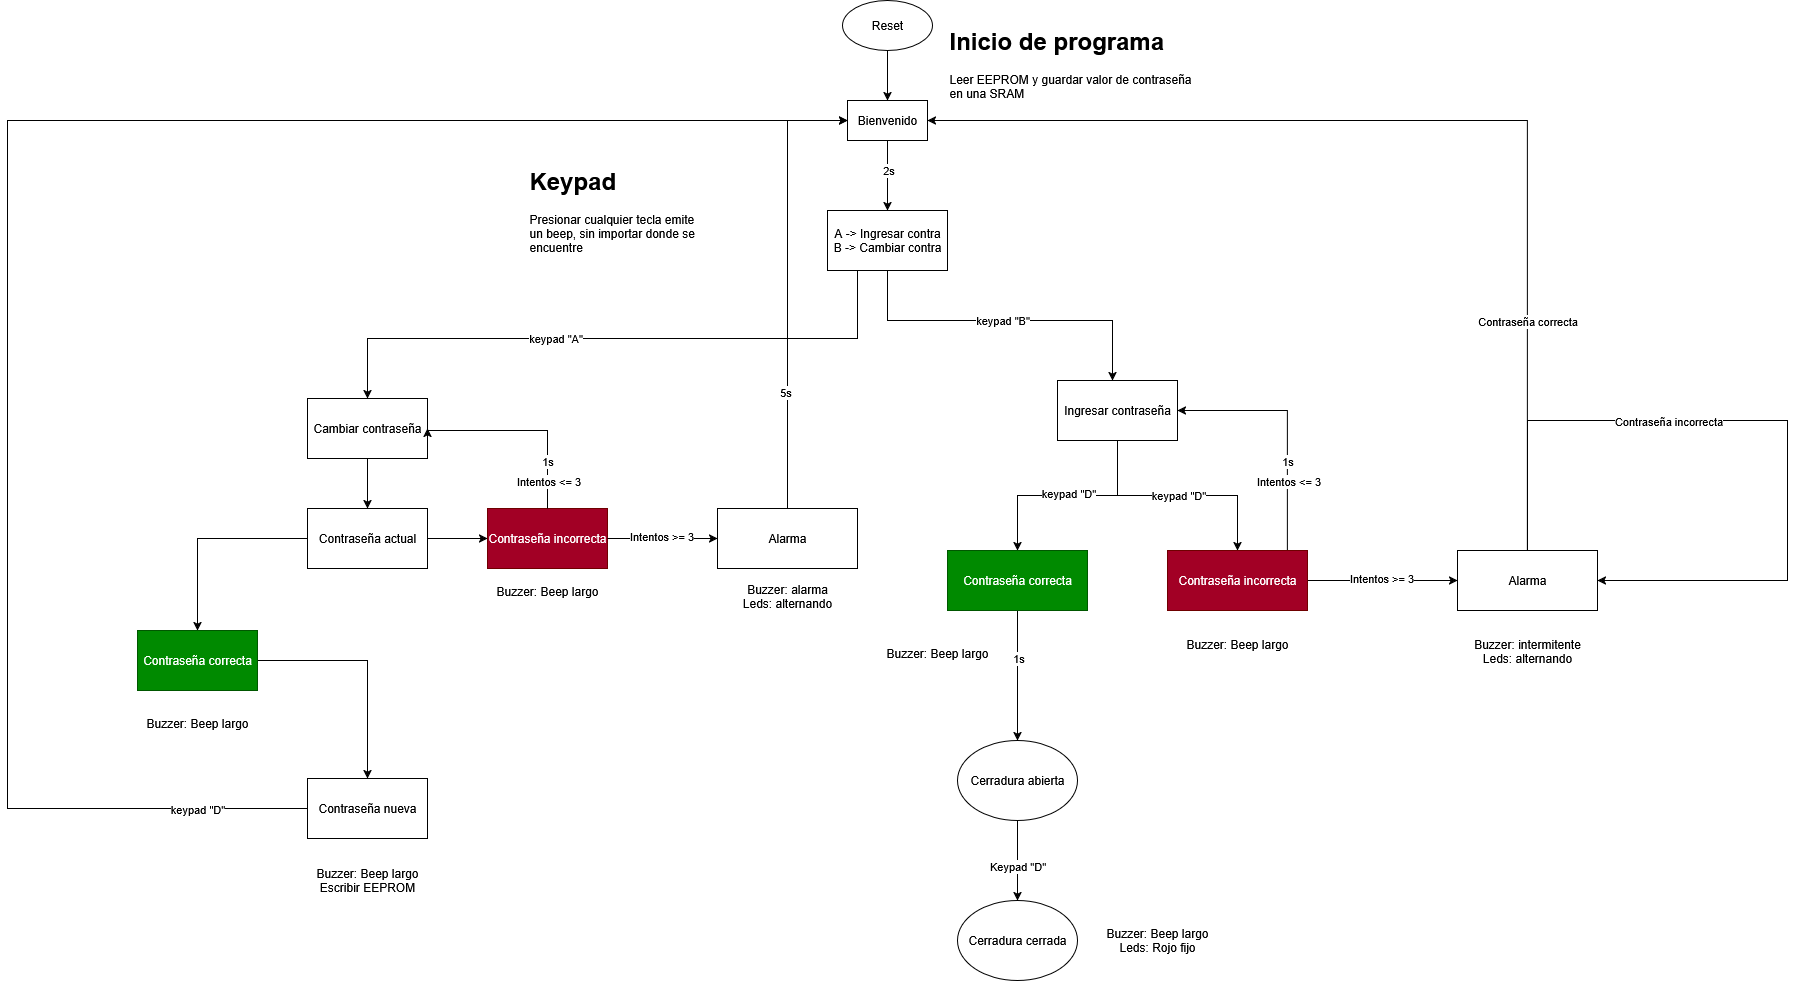
\includegraphics[width=0.9\columnwidth]{anexos/cerradura/DiagramaFlujo.png}
    \caption{Diagrama de flujo. Fuente: elaboración própia}
    \label{fig:lcd_ui}
\end{figure}


Librerias para lcd
\begin{lstlisting}[language=C, caption={Librerias utilizadas para pantalla LCD}]
#include "i2c_master.h"
#include "i2c_master.c"
#include "liquid_crystal_i2c.h"
#include "liquid_crystal_i2c.c"

int main(void){
    LiquidCrystalDevice_t device = lq_init(0x27, 16, 2, LCD_5x8DOTS);
    lq_turnOnBacklight(&device);
	char welcomeText[] = "Bienvenido!";
	lq_print(&device, welcomeText);
    while (1);
}
\end{lstlisting}


Implementacion de tareas
\begin{lstlisting}[language=C, caption={Implementacion de tareas}]
uint32_t millis_counter = 0;

// Mapeo de keypad
const char keypad[4][4] = {
	{'1', '2', '3', 'A'},
	{'4', '5', '6', 'B'},
	{'7', '8', '9', 'C'},
	{'*', '0', '#', 'D'}
};


uint32_t keypad_on_at = 0;
uint8_t keypad_enable = 1;

ISR(TIMER0_OVF_vect){
    millis_counter++;
}

uint32_t millis_now(void) {
    uint32_t m;
    cli();     // disable interrupts
    m = millis_counter;
    sei();     // re-enable
    return m;
}

void keypad_debounce_ms(uint16_t delay_ms){
    keypad_enable = 0;
    keypad_on_at = millis_now() + delay_ms;
}

void keypad_task(void){
    if (!keypad_enable && (millis_now() > keypad_on_at)){
        keypad_enable = 1;
    }
}   

int main(void){
    // main code ...
    while (1){
        keypad_task();
        // loop code ...
    }
}
\end{lstlisting}

Lectura multiplexada de keypad
\begin{lstlisting}[language=C, caption={Funcion de lectura multiplexada de keypad}]
char keypad_scan(void) {
	if (!keypad_enable) return 0;
	
	uint8_t row, col;
	uint8_t cols;
	static uint8_t prevKey; // store for later

	for (row = 0; row < 4; row++) {
		PORTD = (PORTD | 0xF0) & ~(1 << (row + 4));
		_delay_us(5);  
		cols = PIND & 0x0F;  

		for (col = 0; col < 4; col++) {
			if (!(cols & (1 << col)) ) {
				if ((prevKey == keypad[row][col])) return 0;
				
				keypad_debounce_ms(200);
				prevKey = keypad[row][col];
				return keypad[row][col];  
			} 
		}
	}
	prevKey = 0;
	return 0; 
}
\end{lstlisting}

Tarea de alarma
\begin{lstlisting}[language=C, caption={Tarea de alarma}]
 void alarm_task(void){
	if (!alarm_active) return;
	uint32_t now = millis_now();
	
	if (now > alarm_until){
		alarm_active = 0;
		PORTB &= ~(1<<PORTB5);
		led_red_on();
		return;
	}
	
	if (now > alarm_next_toggle){
		alarm_next_toggle = now + ALARM_TOGGLE_MS;
		if (alarm_phase){
			led_red_on();
		} else {
			led_green_on();
		}
		alarm_phase ^= 1;
		
		buzzer_beep(100);
	}
}
\end{lstlisting}

Escritura y lectura de EEPROM
\begin{lstlisting}[language=C, caption={Escritura y lectura de EEPROM}]
#include <avr/eeprom.h>

#define MAX_PASSWORD_LENGTH 6
#define EEPROM_MAGIC 0x42

uint8_t EEMEM ee_magic;                
char EEMEM ee_password[MAX_PASSWORD_LENGTH + 1];

char storedPassword[MAX_PASSWORD_LENGTH + 1] = "123456";
char typedPassword[MAX_PASSWORD_LENGTH + 1];


void eeprom_load_password(void) {
	if (eeprom_read_byte(&ee_magic) != EEPROM_MAGIC) {
		
	eeprom_update_block(
			storedPassword, 
			ee_password, 
			sizeof(storedPassword)
		);

		eeprom_update_byte(&ee_magic, EEPROM_MAGIC);
		} else {
		eeprom_read_block(
			storedPassword, 
			ee_password, 
			sizeof(storedPassword)
		);
	}
}

void eeprom_save_password(const char *pwd) {
	char buf[MAX_PASSWORD_LENGTH + 1];
	strncpy(buf, pwd, MAX_PASSWORD_LENGTH);
	buf[MAX_PASSWORD_LENGTH] = '\0';
	eeprom_update_block(buf, ee_password, sizeof(buf));
}
\end{lstlisting}


Logica de estados
\begin{lstlisting}[language=C, caption={Logica de estados}]
typedef enum { UI_MENU, UI_INGRESO, UI_CAMBIO_ACTUAL, UI_CAMBIO_NUEVA, UI_ABIERTO, UI_ALARMA } ui_state_t;

int main(void){
    while(1){
        char key = keypad_scan();
		if (key) {
			switch (ui_state)
			{
                case UI_MENU: break;
                case UI_INGRESO: break;
                case UI_CAMBIO_ACTUAL: break;
                case UI_CAMBIO_NUEVA: break;
                case UI_CAMBIO_ALARMA: break;
                case UI_CAMBIO_ABIERTO: break;
    }
}
\end{lstlisting}

